\section{Description of the Experiment}
  \label{sec:simultons_experiment}

    \begin{figure}
      \centering     %%% not \center
      \subfigure[Schematic of the three-level V-type atom.]
        {\label{fig:vee_schematic}
        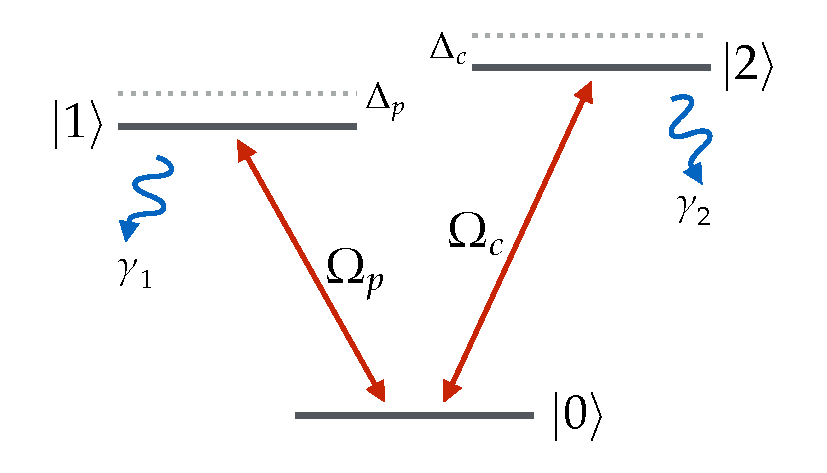
\includegraphics[width=0.4\textwidth]
          {figs/06_simultons/vee_level_diagram.pdf}}
      \subfigure[Hyperfine structure of $^{85}$Rb on the \textsc{d1} and 
                  \textsc{d2} lines, showing angular frequency splittings across hyperfine manifolds.]{\label{fig:rb85_levels}
        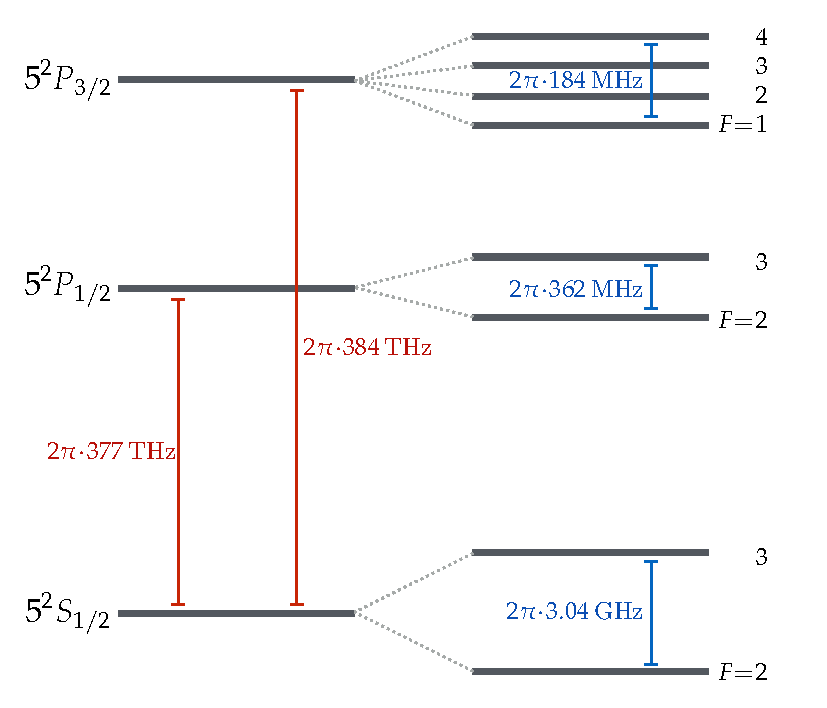
\includegraphics[width=0.4\textwidth]
          {figs/06_simultons/rb85_levels_trim.pdf}}
      \caption{V configuration level diagrams.}
    \end{figure}

    A dense thermal vapour of rubidium atoms in their natural isotopic
    abundances, contained in a thin cell on the order of a micron in length, is
    addressed with two co-propagating monochromatic lasers, forming the V-type
    excitation scheme illustrated in figure \ref{fig:vee_schematic}. The probe
    laser is resonant with the \textsc{d1} transition from the
    $5^2\mathrm{S}_{\nicefrac{1}{2}}$ ground state to the
    $5^2\mathrm{P}_{\nicefrac{1}{2}}$ excited state and the coupling laser is
    resonant with the \textsc{d2} transition coupling the ground state to the
    $5^2\mathrm{P}_{\nicefrac{3}{2}}$ excited state\cite{Arimondo1977,
    Banerjee2007}. The beams are linearly polarised and orthogonal, and
    following propagation they are separated by a polarising beam splitter.

    The $5^2\mathrm{S}_{\nicefrac{1}{2}}$ ground state in rubidium is a doublet
    state split on the order of \unit{GHz}\cite{Arimondo1977}, as shown in
    figure \ref{fig:rb85_levels} for $^{85}$Rb. The experimental carrier
    frequencies are tuned resonant with transitions from the
    $\Ket{5^2\mathrm{S}_{\nicefrac{1}{2}}~F\!=\!3}$ level for $^{85}$Rb and so
    are far-detuned from the other energy level in the doublet. The coupling
    beam is focused to a waist of \unit[${\sim}20$]{$\mu$m} while the probe beam
    is focused more tightly to a waist of \unit[${\sim}10$]{$\mu$m}, which
    minimises variation of the coupling intensity for atoms in the probe
    beam.\cite{Keaveney2013}

    Transmission of the beams through the medium is detected using a fast
    photodiode with a bandwidth of \unit[$8$]{GHz} input to a \unit[$12$]{GHz}
    bandwidth oscilloscope with an effective sampling rate of
    \unit[${\sim}400$]{GS/s}. The oscilloscope is sampling rather than real-
    time, so the data must be averaged over many cycles. Systematic noise is
    recorded by taking measurements with the probe laser off and later removing
    the background from the measured signal.

    The cell windows alter the focusing region of the beams, and so
    spectroscopic measurements are needed to establish accurate Rabi
    frequencies. The Rabi frequency of the coupling beam atom-light interaction
    is measured using the Autler-Townes splitting of the ground states. The Rabi
    frequency of the probe beam is then estimated using the coupling beam as a
    guide.

    Results were taken over a range of peak intensities for the coupling pulse
    of $10$ to \unit[$100$]{mW} and over a vapour temperature range of $200$ to
    $\unit[300]{\textrm{\textdegree C}}$. In all cases the coupling pulse is
    shaped to a short Gaussian profile with a \textsc{fwhm} of \unit[$0.8$]{ns}.
    This shaping is performed by a Pockels cell placed between  two crossed
    Glan-Taylor prisms to rapidly rotate the polarisation of the  beam.

    The experiments were performed and results taken by Kate A. Whittaker and
    James Keaveney. Further details of the experimental setup may be found in
    Keaveney, 2013.\cite{Keaveney2013}

  \subsection{Experimental Results}

    \begin{figure}[h]
      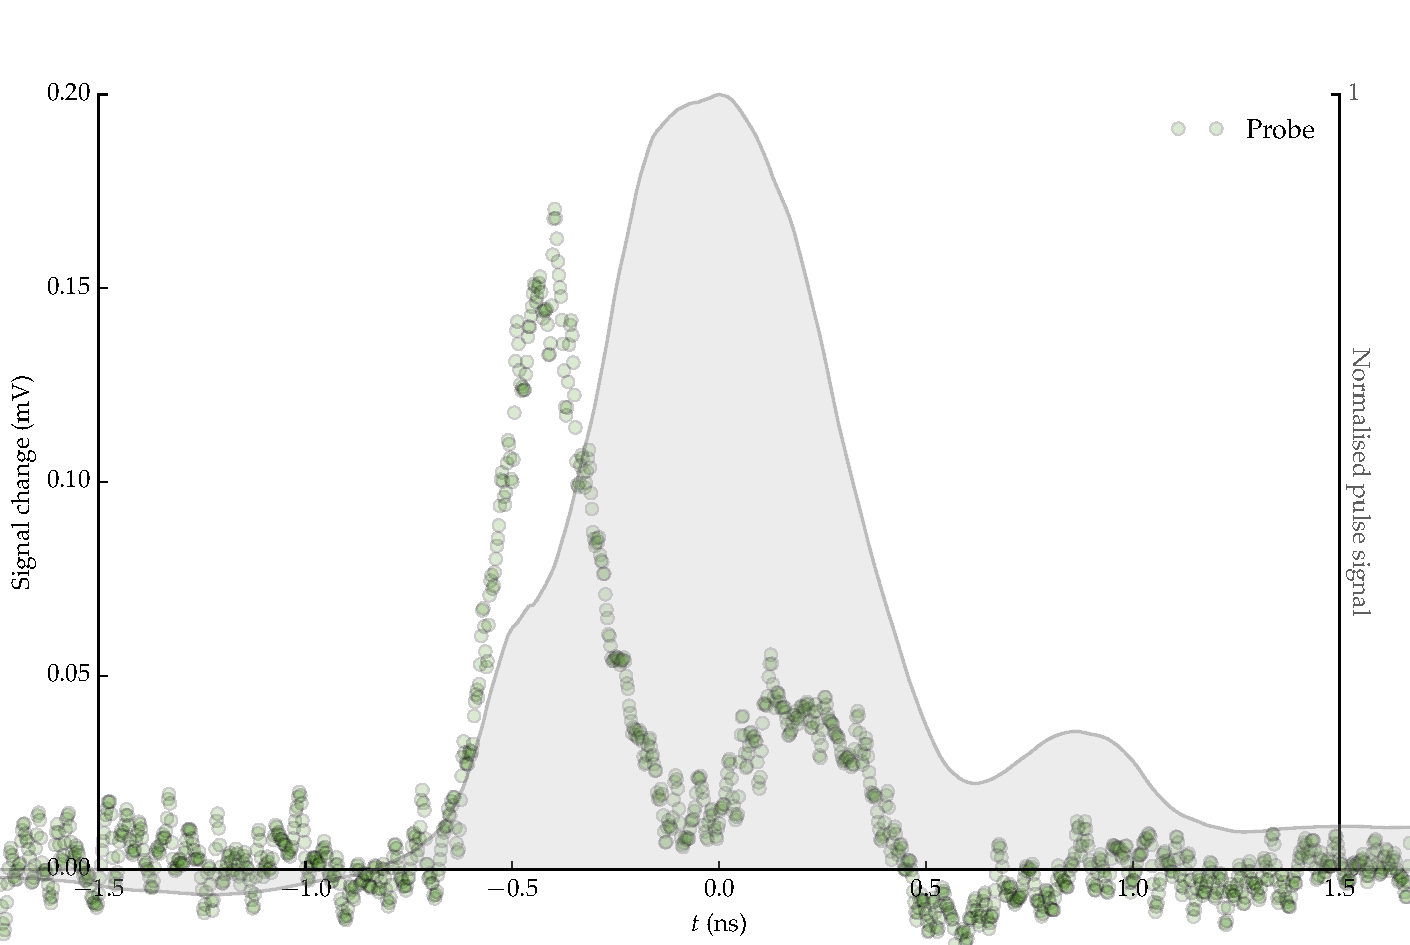
\includegraphics[width=\linewidth]
        {figs/06_simultons/1704_temp_scaled_data_colormap_201C_fig1.pdf}
      \caption{
      Recorded probe transmission against time (green circles). The  resonant
      coupling pulse intensity (grey filled area), shown after it has passed
      through the medium, has a \textsc{fwhm} $t_w = \unit[0.8]{ns}$, a peak
      power of $\unit[82]{mW}$ and is centred at zero. The temperature $T =
      \unit[200]{\textrm{\textdegree C}}$  and the cell length $L = $
      \unit[$2$]{$\mu$m}.
      }
      \label{fig:data_1704_temp_201C}
    \end{figure}

    In figure \ref{fig:data_1704_temp_201C} we see an example result for probe
    field transmission from the experiment described. The change in signal
    detected is plotted against time. In this case the temperature $T =
    \unit[200]{\textrm{\textdegree C}}$ and the cell length $L = $
    \unit[$2$]{$\mu$m}. The coupling pulse has a peak power of $\unit[82]{mW}$
    and is centred at $t\!=\!0$. The coupling pulse plotted is an average of
    many shots, but there is practically no variation in the pulse shape from
    shot to shot.

    We see the probe transmission peak sharply around $\unit[0.5]{ns}$ before
    the maximum of the coupling pulse, which suggests a superluminal propagation
    effect, perhaps due to a negative refractive index in the
    medium.\cite{Keaveney2012}. There is a brief, smaller oscillation before the
    transmission returns to its original level. The input pulse profile applied
    in the experiment has an additional `bump' as an artefact of the way the
    pulse is shaped (this can be seen in the grey pulse shape).

    \begin{figure}[h]
      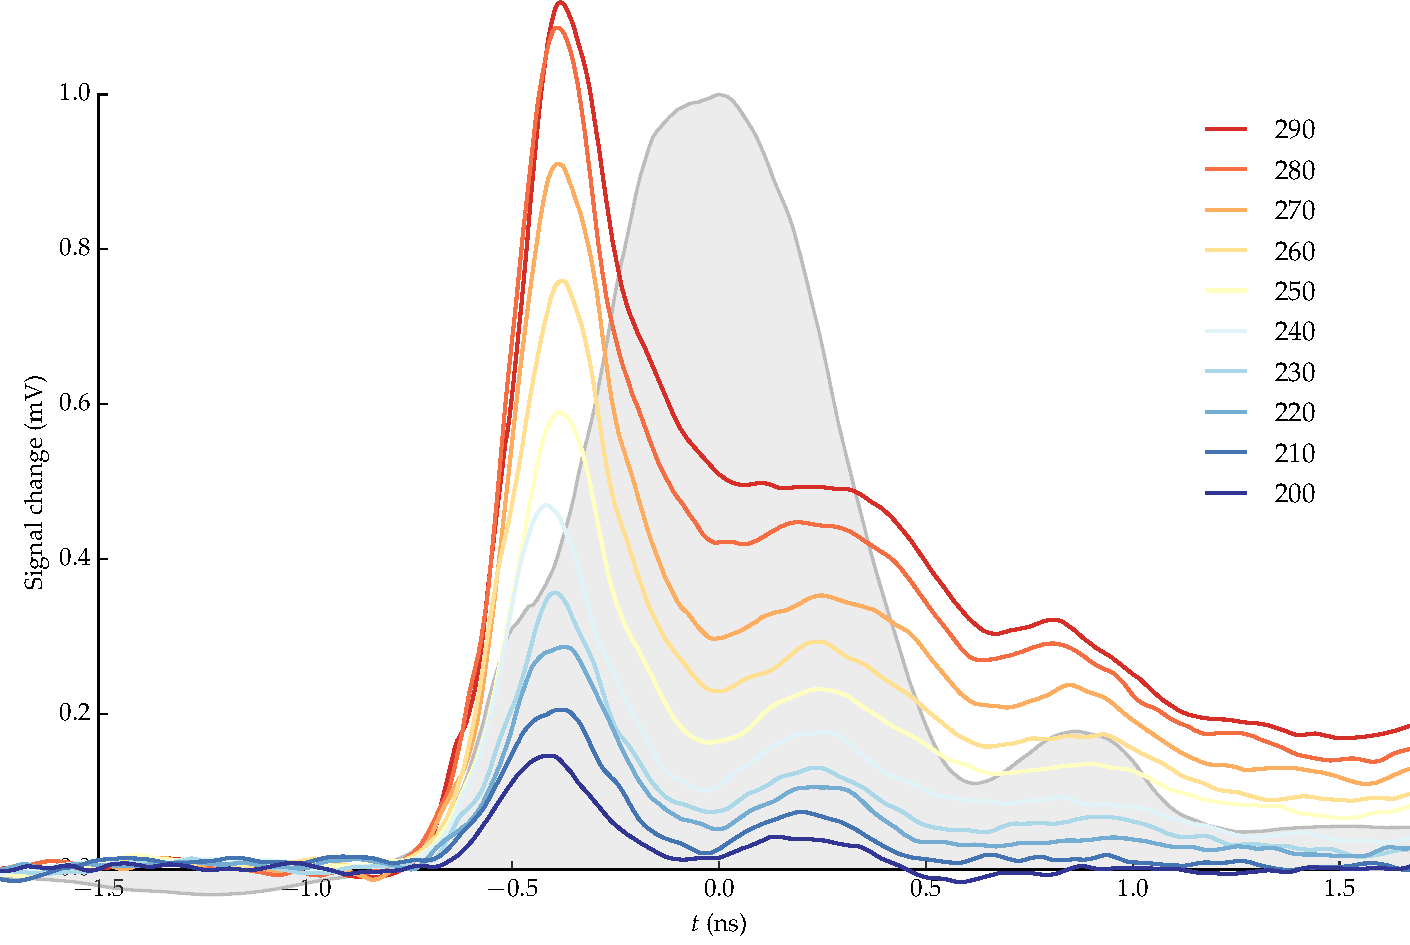
\includegraphics[width=\linewidth]
        {figs/06_simultons/1704_temp_scaled_data_colormap_fig1.pdf}
      \caption{
      Recorded probe signal against time (coloured lines) over a range  of
      temperatures from $T = \unit[200]{\textrm{\textdegree C}}$ to
      $\unit[290]{\textrm{\textdegree C}}$.  The resonant input coupling pulse
      intensity, shown for the experiment at $T = \unit[200]{\textrm{\textdegree
      C}}$ (grey filled area) in each case  has a width $t_w = $
      \unit[$800$]{ps}, is centred at zero and has a peak  optical power of
      \unit[$82$]{mW}. The pulse is shown here normalised for  time reference.
      }
      \label{fig:data_0703_temp_all}
    \end{figure}

    In figure \ref{fig:data_0703_temp_all} we show the recorded change in signal
    over a range of temperatures from $\unit[200]{\textrm{\textdegree C}}$ to
    $\unit[290]{\textrm{\textdegree C}}$. The coupling pulse has a peak optical
    power of \unit[$82$]{mW} and is centred at $t = 0$. For clarity the data has
    been smoothed using a moving average with a triangular weighting function.

    We see that over the range of temperatures investigated at this power, the
    steep early response is consistent in time and that the peak of the response
    increases with temperature in an approximately linear way, with possible saturation of that increase at $\unit[290]{\textrm{\textdegree C}}$.

    In order to understand the distinctive reponse profile of the signal and
    determine the physical principles underlying these results, we will now
    begin building up a theoretical model for the system.
